\documentclass[a4j]{jarticle}			% for platex
\usepackage[dvipdfmx]{graphicx}
\usepackage{multicol}
\usepackage{mathtools}
\usepackage{amsmath, amssymb, amsfonts}


\title{端点を持つ線から描くキャラクターの線画生成}
\author{学籍番号 20C1119 森田大雅}
\date{\today}

\begin{document}
\maketitle % タイトルなどの出力
\small

% \twocolumnは二段組ににしない文章

\begin{abstract}
描画ロボットの研究において、輪郭$\lparen\text{エッジ}\rparen$抽出を行って鉛筆画やハッチング$\lbrack1\rbrack$、インクイラストなどの芸術表現に応用する研究$\lbrack2\rbrack$や機械に手順を示し、そのとおりに描かせる研究$\lbrack3\rbrack$が存在する.
しかし、実際に$\lceil \text{人が描くような描き方} \rfloor$を追求したものは少ないと感じた.
そこで、今回はキャラクターの画像から線画を描く、そしてできるだけ人が描いたような描き方をする描画ロボットを作成する.
\end{abstract}

\begin{multicols}{2} %二段組にする

\section{}

\subsection{人のような描き方の定義}
本研究では$\lbrack4\rbrack$を参考に描き方の方針を進めている.
顔のパーツ配置が定まりやすいという部分に焦点を当てた.
手順としては、最初に顎を描き、次に髪などの頭上部、そして首、
\begin{enumerate}
	\setlength{\parskip}{0cm}
	\setlength{\itemsep}{0cm}
	\item \ 顎\\
	\item \ 頭上部$\lparen \text{髪、頭など} \rparen$\\
	\item \ 首 \\
	\item \ 目、鼻、耳\\
	\item \ その他$\lparen \text{胴体や服など} \rparen$ \\
\end{enumerate} 
これは顎や髪、頭などの頭上部から描き、次に目や鼻、耳などの細部を描くという順序である.
理由は全体を描いてから、細部を描いた方が目や鼻の位置を定めやすいからである.

\section{システム構成}
このシステムは主に3つから構成されている. 
1つが画像から輪郭を抽出する.
2つが抽出した画像から線の経路を求める.
3つが線の経路をもとに実機を動かして描かせる.

\subsection{処理の流れ}
細かな処理の流れは以下の通りである.\\ 
\begin{enumerate}
	\setlength{\parskip}{0cm} % 段落間
	\setlength{\itemsep}{0cm} % 項目間
	\item 平滑化\\
	\item エッジ抽出\\
	\item 細線化\\
	\item 端点の検出\\
	\item 経路を求め、移動すべき座標を取得\\
	\item 取得した座標をもとに機械に描かせる\\
\end{enumerate}

\subsection{エッジ抽出}
輪郭抽出にはエッジ抽出が一般的に行われる.
ソーベルフィルタやケニーのエッジ検出なども検討したが、実際に試したところラプラシアンフィルタをエッジ抽出に用いることにした.

% ここに図を挿入する

\subsection{細線化}
線の経路の求め方は、ある線の画素から隣に線の画素があるかを探して、移動してを繰り返すものとなっている.
そのため、線を一本に単純化してある方が線をたどるのに容易であるため細線化を行う.

 % \subsection{線のたどり方}  概要なので割愛

\subsection{端点を持つ線から描く理由}
端点を検出して描くのには2つの理由がある.
線画を生成する過程で繋がっているはずの線が途切れてしまうというのが一つの理由である.
それは平滑化、エッジ抽出、細線化処理を施すからである.

\end{multicols}
\section{ロボットの機構}
本研究で用いるロボットは3軸のマニピュレータロボットである.
下の図1のようにアームの先端、姿勢の関節角を$\theta_1, \theta_2, \theta_3$、各リンクの長さ$l_1, l_2, l_3, l_4$とし、逆運動学問題を解く.
またリンク座標系を定める方法として、DH記法(Denavit-Hartenberg記法)を用いる.


\begin{figure}[htbp]
\begin{center}
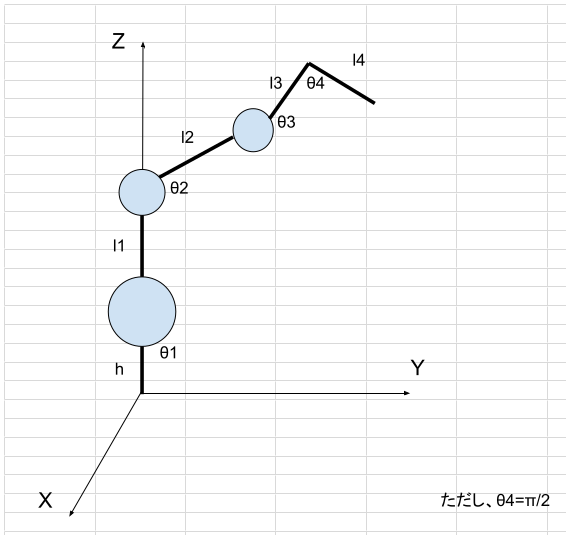
\includegraphics[width=100mm]{/home/hiromasa/ros2_ws/Memo/tex/img/img1.png}
\caption{リンク座標系}
\end{center}
\end{figure}



\begin{multicols}{2} %二段組にする
座標系0から3への座標変換行列 
$$
	^{0}T_{3}=^{0}T_{1} ^{1}T_{2} ^{2}T_{3} \\
$$
\begin{equation*}
	\begin{array}{cc}
		=
		\left( 
			\begin{array}{cccc}
				C_1C_{23} & -C_1S_{23} & 0 & l_2C_1S_2 \\
				S_1C_{23} & -S_1S_{23} & 0 & l_2S_1S_2 \\
				-S{23} & -C_{23} & -1 & l_2C_2 + l_1 \\
				0 & 0 & 0 & 1 
			\end{array}
		\right)
	\end{array}
\end{equation*}

ただし、
\begin{equation*}
	\left(
	\begin{split}
		C_{23} = cos\theta_2cos\theta_3-sin\theta_2sin\theta_3\\
		S_{23} = sin\theta_2cos\theta_3+cos\theta_2sin\theta_3	
	\end{split}
	\right)
\end{equation*}

手先ベクトル
\tiny
\begin{equation*}
	\begin{array}{cccc}
		\left( 
			\begin{array}{cccc}
				1 & 0 & 0 & l_4\\
				0 & 1 & 0 & 0\\
				0 & 0 & 1 & 0\\
				0 & 0 & 0 & 1 
			\end{array}
		\right)
		\left( 
			\begin{array}{cccc}
				1 & 0 & 0 & 0\\
				0 & 1 & 0 & -l_3\\
				0 & 0 & 1 & 0\\
				0 & 0 & 0 & 1 
			\end{array}
			\right)
		=
		\left( 
		\begin{array}{cccc}
			1 & 0 & 0 & l_4\\
			0 & 1 & 0 & -l_3\\
			0 & 0 & 1 & 0\\
			0 & 0 & 0 & 1 
		\end{array}
		\right)
	\end{array}
\end{equation*}
\small
より手先までの座標変換行列$^{0}P_{r}$が以下のように求まる.
\tiny
\begin{equation*}
	\begin{array}{cc}
		\left( 
			\begin{array}{cccc}
				C_1C_{23} & -C_1S_{23} & 0 & l_4C_1C_{23}+l_3C_1S_{23}+l_2C_1S_2 \\
				S_1C_{23} & -S_1S_{23} & 0 & l_4S_1C_{23}+l_3S_1S_{23}+l_2S_1S_2 \\
				-S{23} & -C_{23} & -1 & -l_4S_{23}+l_3C_{23}+l_2C_2+l_1 \\
				0 & 0 & 0 & 1 
			\end{array}
		\right)
	\end{array}
\end{equation*}
\small
そしてこの行列から手先の位置x, y, zは以下のように求まる.
\begin{equation*}
	\left\{
		\begin{array}{c}
		\begin{split}
			&x=C_1(l_4C_{23}+l_3S_{23}+l_2S_2)\quad(3.1) \\
			&y=S_1(l_4C_{23}+l_3S_{23}+l_2S_2)\quad(3.2) \\
			&z-l_1=-l_4S_{23}+l_3C_{23}+l_2C_2\quad(3.3) \\
		\end{split}
	\end{array}
	\right.
\end{equation*}
これらを解くと
\tiny
\begin{equation*}
\left\{
	\begin{array}{c}
	\begin{split}
		&\theta_1=\frac{1}{2}cos^{-1}\biggl( \frac{x^2-y^2}{x^2+y^2} \biggr) \\
		&\theta_3= cos^{-1}\biggl( \frac{1}{\sqrt{a^2+b^2}}\biggr) + cos^{-1}\biggl( \frac{b}{\sqrt{a^2+b^2}}\biggr)\\
		&\theta_2= cos^{-1}\biggl( \frac{1}{\sqrt{c^2+d^2}}\biggr) + cos^{-1}\biggl( \frac{d}{\sqrt{c^2+d^2}}\biggr)
	\end{split}
	\end{array}
\right.
\end{equation*}
\small
ただし、
\begin{equation*}
	\left(\quad
	\begin{split}
		&a=\frac{2l_2}{l_4^2+l_3^2+l_2^2-\{x^2+y^2+(z-l_1^2)^2 \} }l_4\\
		&b=\frac{2l_2}{l_4^2+l_3^2+l_2^2-\{x^2+y^2+(z-l_1^2)^2 \} }l_3\\
		&c=\frac{l_2S_3-l_4}{ C_3(z-l_1)+S_3\bigl(\frac{x}{C_1}\bigr)}\\
		&d=\frac{l_2S_3+l_3}{ C_3(z-l_1)+S_3\bigl(\frac{x}{C_1}\bigr)}
	\end{split}
	\quad\right)
\end{equation*}

\section{参考文献}

\begin{enumerate}
\item \lbrack 1\rbrack \ Raspberry Piを利用した肖像画描画ロボット :$ \lceil Pankraz Piktograph \rfloor$ \\
\item \lbrack 2\rbrack \ XDoG: An Xtended difference-of-Gaussians compendium \\
\item \lbrack 3\rbrack \ ロボットによる描画行為の再現\\
\item \lbrack 4\rbrack \ 出版:主婦の友社\ $\lceil \text{小河原智子の似顔絵入門} \rfloor$\\
\item 広瀬\ 茂男\ 著\ 機械工学選書\ 裳華房\ ロボット工学-機械システムのベクトル解析-\\
\item 細田\ 耕著\ 実践ロボット制御-基礎から動力学まで- \\
\end{enumerate}

\end{multicols}

\end{document}
